\documentclass[../../main.tex]{subfiles}
\begin{document}

{\bf [解答]}

\begin{figure}[htb]
  \centering
  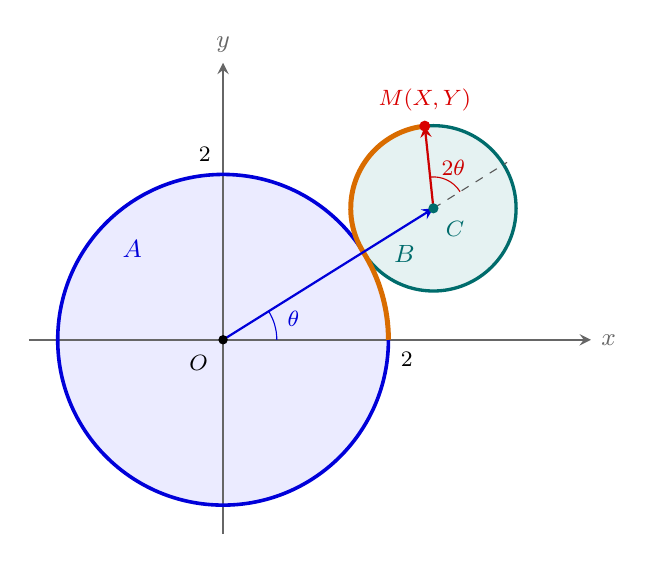
\begin{tikzpicture}[x=1.05cm, y=1.05cm, >=stealth, every node/.style={font=\small}]
    % Fixed circle A: center O(0,0), radius 2
    % Rolling circle B: center C(3 cos theta, 3 sin theta), radius 1, theta = 32 deg
    \pgfmathsetmacro{\th}{32}
    \pgfmathsetmacro{\cx}{3*cos(\th)}
    \pgfmathsetmacro{\cy}{3*sin(\th)}
    \pgfmathsetmacro{\tx}{2*cos(\th)}
    \pgfmathsetmacro{\ty}{2*sin(\th)}
    \pgfmathsetmacro{\mx}{\cx+cos(3*\th)}
    \pgfmathsetmacro{\my}{\cy+sin(3*\th)}
    \coordinate (O) at (0, 0);
    \coordinate (C) at (\cx, \cy);
    \coordinate (T) at (\tx, \ty);
    \coordinate (M) at (\mx, \my);
    \coordinate (Cref) at ({\cx+1.05*cos(\th)}, {\cy+1.05*sin(\th)});

    % 固定円板 A と転がる円板 B
    \fill[blue!8] (O) circle (2);
    \fill[teal!10] (C) circle (1);
    \draw[->, thick, gray!80!black] (-2.35, 0) -- (4.45, 0) node[right] {$x$};
    \draw[->, thick, gray!80!black] (0, -2.35) -- (0, 3.35) node[above] {$y$};

    \draw[line width=1.3pt, blue!85!black] (O) circle (2);
    \draw[line width=1.2pt, teal!85!black] (C) circle (1);

    % 転がった弧の強調（滑らない条件: 2\theta = 1 \cdot \angle TCM）
    \draw[line width=1.8pt, orange!85!black] (2, 0) arc[start angle=0, end angle=\th, radius=2];
    \draw[line width=1.8pt, orange!85!black] (T) arc[start angle={180+\th}, end angle={3*\th}, radius=1];

    % 動径 OC, 延長線, CM
    \draw[thick, blue!85!black, ->] (O) -- (C);
    \draw[dashed, gray!70!black] (C) -- (Cref);
    \draw[thick, red!80!black, ->] (C) -- (M);

    % 角度の弧
    \draw[thin, blue!85!black] (0.65, 0) arc[start angle=0, end angle=\th, radius=0.65];
    \node[font=\footnotesize, blue!85!black] at (0.85, 0.25) {$\theta$};
    \draw[thin, red!80!black] ({\cx+0.38*cos(\th)}, {\cy+0.38*sin(\th)})
    arc[start angle=\th, end angle={3*\th}, radius=0.38];
    \node[font=\footnotesize, red!80!black] at ({\cx+0.55*cos(2*\th)}, {\cy+0.55*sin(2*\th)}) {$2\theta$};

    % 点とラベル
    \node[circle, fill, inner sep=1.2pt] at (O) {};
    \node[below left=2pt, font=\footnotesize] at (O) {$O$};
    \node[circle, fill=teal!85!black, inner sep=1.3pt] at (C) {};
    \node[below right=1pt, font=\footnotesize, teal!85!black] at (C) {$C$};
    \node[circle, fill=red!85!black, inner sep=1.4pt] at (M) {};
    \node[above=2pt, font=\footnotesize, red!85!black] at (M) {$M(X,Y)$};
    \node[below right=1pt, font=\footnotesize] at (2, 0) {$2$};
    \node[above left=1pt, font=\footnotesize] at (0, 2) {$2$};
    \node[font=\small, blue!85!black] at (-1.1, 1.1) {$A$};
    \node[font=\small, teal!85!black] at ({\cx-0.35}, {\cy-0.55}) {$B$};
  \end{tikzpicture}
  \caption{固定円板 $A$ の周上を滑らずに転がる円板 $B$ と点 $M(X,Y)$ の位置}
  \label{fig:1974_5_rolling_circles}
\end{figure}

\subparagraph{(1)}

グラフから
\begin{align}
  \overrightarrow{OM} = \overrightarrow{OC} + \overrightarrow{CM}
\end{align}
で，各項計算すると
\begin{align}
  \overrightarrow{OC} = 3
  \begin{pmatrix} \cos\theta \\ \sin\theta
  \end{pmatrix}
  \quad
  \overrightarrow{CM} =
  \begin{pmatrix} \cos3\theta \\ \sin3\theta
  \end{pmatrix}
\end{align}
だから，三倍角の公式$\cos3\theta=4\cos^3\theta-3\cos\theta, \sin 3\theta=-4\sin^3\theta+3\sin\theta$より
\begin{align}
  \begin{cases}
    X=3\cos\theta+\cos 3\theta=4\cos^3\theta \\
    Y=3\sin\theta+\sin 3\theta=6\sin\theta-4\sin^3\theta
  \end{cases} \label{eq:1}
\end{align}
である．$\cdots$(答)

\subparagraph{(2)}

\cref{eq:1}の両辺を$\theta$で微分して
\begin{align}
  \begin{cases}
    X'=-12\cos^2\theta\sin\theta \\
    Y'=6\cos\theta(1-2\sin^2\theta) = 6\cos\theta(2\cos^2\theta-1)
  \end{cases} \label{eq:2}
\end{align}
であり，下表を得る．

\begin{table}[htb]
  \centering
  \caption{$\theta$ の変化に対する $(X,Y)$ の増減表}
  \label{tab:1974_5_variation}
  \renewcommand{\arraystretch}{1.35}
  \begin{tabular}{|c|c|c|c|c|c|}
    \hline
    $\theta$ & $0$ & $\cdots$ & $\dfrac{\pi}{4}$ & $\cdots$ & $\dfrac{\pi}{2}$ \\
    \hline
    $X'$ & $0$ & $-$ & $-$ & $-$ & $0$ \\
    \hline
    $Y'$ & $+$ & $+$ & $0$ & $-$ & $0$ \\
    \hline
    $(X,Y)$ & $(4,0)$ & $\nwarrow$ & $(\sqrt{2},2\sqrt{2})$ & $\swarrow$ & $(0,2)$ \\
    \hline
  \end{tabular}
\end{table}

\begin{figure}[htb]
  \centering
  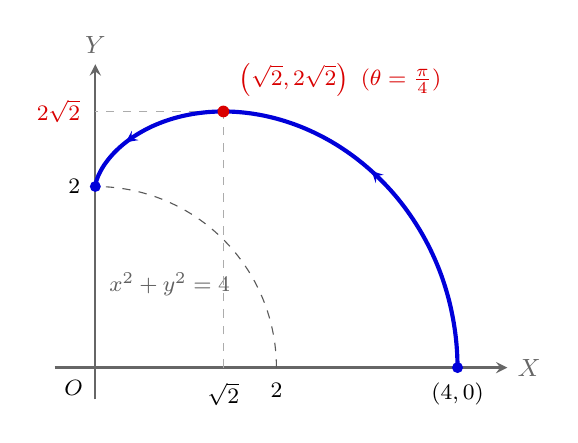
\begin{tikzpicture}[x=1.15cm, y=1.15cm, >=stealth, every node/.style={font=\small}]
    % Parametric curve: X = 4 cos^3(t), Y = 6 sin(t) - 4 sin^3(t) for 0 <= t <= 90 deg
    \coordinate (O) at (0, 0);
    \coordinate (P0) at (4, 0);
    \coordinate (Pmax) at ({sqrt(2)}, {2*sqrt(2)});
    \coordinate (P1) at (0, 2);

    \draw[->, thick, gray!80!black] (-0.45, 0) -- (4.55, 0) node[right] {$X$};
    \draw[->, thick, gray!80!black] (0, -0.35) -- (0, 3.35) node[above] {$Y$};

    % 円板 A (第1象限)
    \draw[dashed, gray!70!black, domain=0:90, samples=60] plot ({2*cos(\x)}, {2*sin(\x)});
    \node[font=\footnotesize, gray!75!black] at (0.82, 0.92) {$x^2+y^2=4$};

    % 投影破線
    \draw[dashed, gray!65] ({sqrt(2)}, 0) -- (Pmax) -- (0, {2*sqrt(2)});

    % M の描く曲線
    \draw[line width=1.5pt, blue!85!black, domain=0:90, samples=100, smooth]
    plot ({4*(cos(\x))^3}, {6*sin(\x)-4*(sin(\x))^3});

    % 進行方向の矢印
    \draw[->, thick, blue!85!black] ({4*(cos(22))^3}, {6*sin(22)-4*(sin(22))^3})
    -- ({4*(cos(24))^3}, {6*sin(24)-4*(sin(24))^3});
    \draw[->, thick, blue!85!black] ({4*(cos(62))^3}, {6*sin(62)-4*(sin(62))^3})
    -- ({4*(cos(64))^3}, {6*sin(64)-4*(sin(64))^3});

    % 点とラベル
    \node[circle, fill=blue!85!black, inner sep=1.4pt] at (P0) {};
    \node[below=2pt, font=\footnotesize] at (P0) {$(4,0)$};
    \node[circle, fill=red!85!black, inner sep=1.5pt] at (Pmax) {};
    \node[above right=2pt, font=\footnotesize, red!85!black] at (Pmax)
    {$\left(\sqrt{2},2\sqrt{2}\right)\ (\theta=\frac{\pi}{4})$};
    \node[circle, fill=blue!85!black, inner sep=1.4pt] at (P1) {};
    \node[left=2pt, font=\footnotesize] at (P1) {$2$};
    \node[below=2pt, font=\footnotesize] at (2, 0) {$2$};
    \node[below=2pt, font=\footnotesize] at ({sqrt(2)}, 0) {$\sqrt{2}$};
    \node[left=2pt, font=\footnotesize, red!85!black] at (0, {2*sqrt(2)}) {$2\sqrt{2}$};
    \node[below left=1pt, font=\footnotesize] at (O) {$O$};
  \end{tikzpicture}
  \caption{$0\le\theta\le\dfrac{\pi}{2}$ における点 $M(X,Y)$ の軌跡}
  \label{fig:1974_5_trajectory}
\end{figure}

従って$Y$の最大値は$\max Y=2\sqrt{2}$である．$\cdots$(答)

\subparagraph{(3)}

求める孤長$L$とすると，\cref{eq:2}より
\begin{align}
  L&=\int_0^{\pi/2}\sqrt{X'^2+Y'^2}\,d\theta \\
  &=\int_0^{\pi/2}\sqrt{144\cos^4\theta\sin^2\theta+36\cos^2\theta(2\cos^2-1)^2}\,d\theta \\
  &=\int_0^{\pi/2}\sqrt{36\cos^2\theta}\,d\theta \\
  &=\int_0^{\pi/2}6\cos\theta\,d\theta \quad (\because \cos\theta\ge0)\\
  &=6
\end{align}
である．$\cdots$(答)
\newpage
\end{document}
